\chapter{Related Work}

\begin{itemize}
    \item what has been done
    \item approaches to our problem
    \item mention models we will use
\end{itemize}

In this chapter we present existing approaches to text embedding and discuss
their advantages and disadvantages for semantically representing longer pieces
of texts.

We split the existing models into categories based on their architecture. First
we present \emph{bag-of-words} (\emph{BOW}) methods, which view input texts as
unordered set of words. From these methods we mention TF-IDF and Paragraph
Vector (PV) models. Second, we describe transformer-based models, which
rely on the Transformer architecture. In this category we mention Longformer,
BigBird, SBERT and CDLM. Finally, we describe hierarchical models such as SMITH.


%TODO: organize this differently
\section{Models}

In this section we describe a set of benchmark models our model will be compared
to. All of the benchmark models are able to map a continuous piece of text to a
dense vector representation. This was a requirement as the aim of the evaluation
is to compare different text embeddings. Otherwise we aimed to select a variety
of models with different architectures, learning algorithms and learning tasks.

\subsection{Paragraph Vector}

Paragraph Vector (also known as Doc2Vec) introduced in \cite{le2014distributed},
combines slightly altered DBOW and DM architectures previously used by Word2Vec
in \cite{mikolov2013efficient}. As seen in Figure~\ref{fig:pv-dm_pv-dbow} the
model's versions of DBOW and DM architectures, called PV-DBOW and PV-DM,
incorporate paragraph's identifier. This allows the architectures to store the
information about the input paragrahs, which is then used as the paragraph's
embedding. The final paragrpah embedding is linear combination of the
representations of both architectures. Note that, a paragrpah can be any piece
of continuous text.

TODO: my own graphic here

\begin{figure}[h]
    \centering
    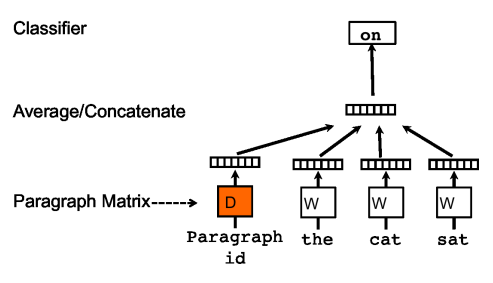
\includegraphics[width=0.4\textwidth]{./img/pv-dm.png}
    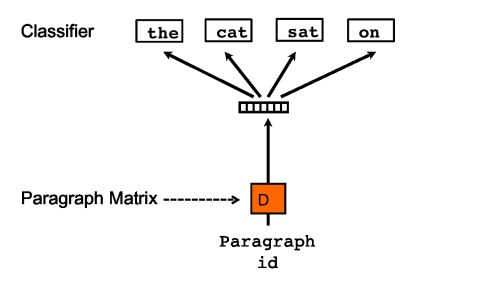
\includegraphics[width=0.4\textwidth]{./img/pv-dbow.png}
    \caption{PV-DM and PV-DBOW architectures.\label{fig:pv-dm_pv-dbow}}
\end{figure}

Paragraph Vector is trained using language modelling --- both architectures should
predict a word which is probable in the given context. In PV-DM the context is
paragraph id and the neighbouring words, in PV-DBOW the context is only the
pragraph id.

Paragraph Vector's advantage is its small size and therefore quick learning.
Moreover it is able to process paragraphs of all lengths. The disadvantage is
that the embedding must be learned even during inference.

\subsection{SBERT}

Sentence-BERT (or SBERT for short) introduced in \cite{reimers2019sentence}, is
a composition of a BERT-like model with pooling layer above its final hidden
states. This architecture is common for sequence classification using a
transformer model. SBERT differs from these simpler approaches, by finetuning on
NLI datasets using siamiese networks. The training setup is depicted in
Figure~\ref{fig:sbert_siemese}. After such training the STS scores of SBERT
embeddings significantly increases.

\begin{figure}
    \centering
    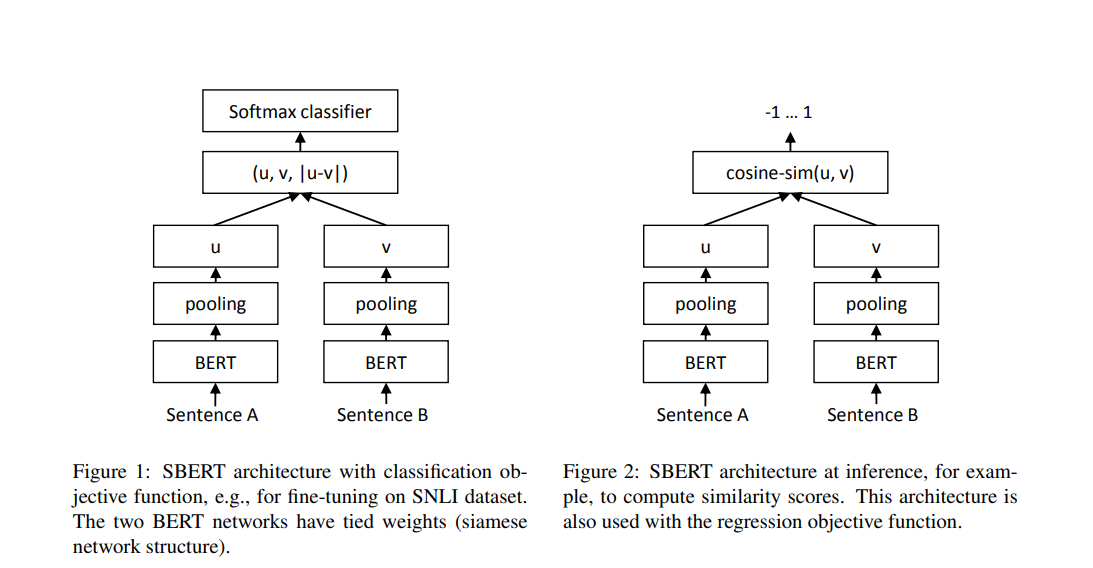
\includegraphics[width=0.9\textwidth]{./img/sbert_pairs_architectures.png}
    \caption{SBERT architecture with siamiese
    networks.\label{fig:sbert_siemese}}
\end{figure}

The disadvantage of SBERT is its inability to process longer pieces of texts.
The workaround is to either truncate the input or to average multiple embeddings
produced by a sliding window over the input. Both approaches limit the model's
ability to see the document as a whole, which could impair the quality of the
produced embeddings.

\subsection{Longformer}

Longformer introduced in \cite{beltagy2020longformer}, is a transformer with
sparse attention matrix. Whereas in traditional transformer we see dense
attention matrix --- every token ``attends'' to every other token, in
Longformer's attention every token ``attends'' only to selected few global
tokens and neighbouring tokens. Example of such sparse attention matrix is
depicted in Figure~\ref{fig:longformer_sparse_att}. This allows Longformer to
process inputs in linear time of the input length. Thus Longformer is able to
process inputs up to 4096 tokens long.

TODO: maybe comparison to normal dense attention

\begin{figure}[h]
    \centering
    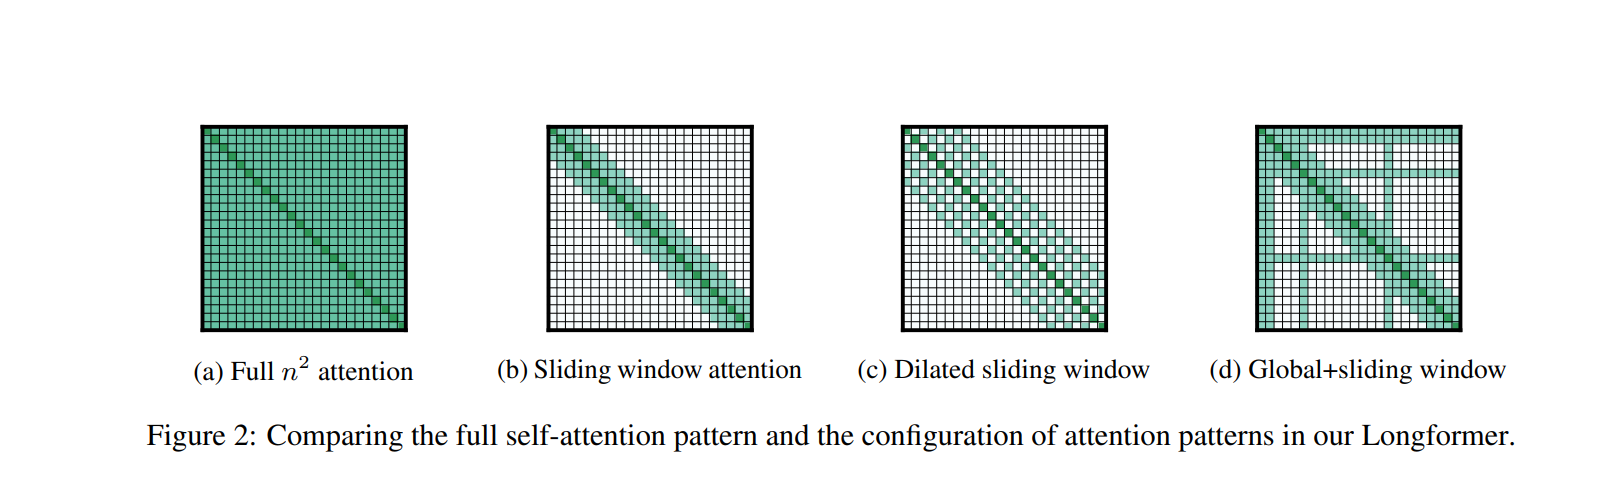
\includegraphics[width=0.9\textwidth]{./img/longformer_attention.png}
    \caption{Longformer attention matrix.\label{fig:longformer_sparse_att}}
\end{figure}

While sparse attention matrix allows Longformer to process longer texts, it also
limits its computational power. \cite{zaheer2020big} show that with sparse
attention we need more layers to match the power of a dense attention matrix.

To produce input embeddings we average the embeddings of last hidden states.

TODO: training

\subsection{BigBird}

TODO: how is it different from longformer




